\chapter{Electron beam lithography on the TU Delft Kavli Nanolab Raith EBPG 5000+ and 5200, using \textit{LayoutBEAMER} and \textit{cjob}}
\label{app:ebeam}
\clearpage

\section{Ebeam alignment}
When writing patterns onto a chip, you usually will specify the location of where on the chip you want your pattern to be.

\subsection{Single layer exposure}
If your exposure is the first and only one on this chip, you can simply note down the coordinates of two opposite corners of your chip, from which you can calculate the chip center. This point you can then give the ebeam as location for your job exposure.

\subsection{Alignment of various layers to each other}
It is always good to add alignment marks to your pattern in case you will want to do another ebeam step on your sample. Obviously, for multiple steps you will want to have a very good alignment of the individual steps with respect to the previous layers. There are various types of ebeam markers available in cjob. In our lab we usually make use of rectangular markers that are 20um by 20um. Depending on the polarity, i.e. whether these will be elevated (positive) or holes (negative), these markers are called RP20 or RN20, respectively.
Depending on how good your alignment needs to be you might do with just one set of markers

\subsubsection{How marker search works}
There are two ways for searching for and aligning to markers:
\begin{enumerate}
	\item Manually: This is only possible in \lstinline|operator| mode: Move to the marker positions (e.g. via \lstinline|almic2ebpg| or directly via \lstinline|mpos|, turn on the SEM and align to the markers. This way you can align to any recognizable structure with known position. You should only use this if the machine cannot recognize your markers (due to dirt on top)
	\item Automatically: you should always use this because the machine will be better than you. In your cjob file you need to tell the ebeam which marker type (RECT for rectangular metallic, TOPO for topographic makers), POSitive or NEGative tone and what size they are. Arnold suggests that best markers to use are rectangles; the typical size is \SI{20}{\micro\meter}, maximum size \SI{100}{\micro\meter}. Crosses can also be used, but alignment is harder
\end{enumerate}

The default marker, as they are on the holders, are \lstinline|RECT POS 20,20|, or \lstinline|RP20|.
For an automatic marker search, the ebeam starts at the specified position and scans outwards in a rectangular spiral, while at the same time measuring the contrast. In the end, once it measures a step of significant contrast and length that matches to the specified marker type, it will stop. If it doesn't find anything, it will abort after a certain radius.
The marker search parameters are:
\begin{itemize}
	\item expected contrast \lstinline|CONTRA| (default \SI{97}{\percent})
	\item maximum radius \lstinline|ISRAD| (default 50um, max half a scan field)
	\item step \lstinline|ISXSTP, ISYSTP| (default \SI{30}{\percent} marker size)
\end{itemize}
 
Note that you should keep a free area (recommended are >\SI{100}{\micro\meter}) around each marker. This will help to avoid search failures due to confusion with other features. Also note that your markers should not be too close to your patterns, since marker search is at a very high dose, so you are constantly exposing the resist.

\subsubsection{How many markers are needed?}
At least three markers are needed for correcting rotation, shift and scaling. It is recommended however that you use (at least) four markers to also account for shear and perspective distortion.

\subsubsection{General rules for highest alignment}
For the highest possible alignment precision (specs of the EBPG5000 and 5200 are below \SI{10}{\nano\meter}) these steps should be followed:
\begin{itemize}
	\item Do not use manual marker search. The machine is always better than you.
	\item Never use markers twice. Especially small beams can be extremely sensitive to any dirt on your markers, so make sure you have enough backup markers (at least one set per step)
	\item Do rough and fine alignment: Do one alignment on R20 at the exposure level, one R20 alignment at the layout level, and one R10 alignment at the pattern level
	\item Use small markers for fine alignment (i.e. RN10/RP10 as the last alignment step)
	\item Put your pattern inside your markers
	\item The pattern should be within \SI{500}{\micro\meter} of each marker, i.e. do space your markers further apart than \SI{1}{\milli\meter}
\end{itemize}

\subsubsection{Rough alignment}
\begin{itemize}
	\item If the ebeam cannot find your markers, you might consider manual marker search (set marker type to \lstinline|JOY| and run job as \lstinline|operator|). Alignment will be significantly worse in this case, but at least you might be able to expose
	\item Dirt on your markers can lead to the ebpg not recognizing them or, worse, misinterpreting edges, so that your pattern will be scaled or even misaligned
	\item For alignment down to \SI{1}{\micro\meter} (rough estimation), it is not necessary to put all of your pattern inside an area enclosed by your markers. For a \SI{10x10}{\milli\meter} chip, you can for example place your markers at $\pm\SI{3000}{\micro\meter},\pm\SI{4000}{\micro\meter}$ and still expose and align all the way to the outside of the chip edge (with worse alignment the further outside the marker area you expose)
\end{itemize}

\subsection{Example workflow of high-accuracy alignment on a big chip}
This is an example workflow from Felix' device 1809.3. It is a \SI{22x22}{\milli\meter} chip used for four \SI{10x10}{\milli\meter} chips, each with three DC bias cavities. At the end of two of each cavities per chip, there is a graphene JJ with several ebeam steps, which require high-accuracy alignment. As an example we will cover the alignment for the third exposure, "shapingARP". Note that every single pattern is different from the others, so we cannot simply use the same patterns for each junction, but require individual patterns, hence the huge number of patterns and colors.

\subsubsection{First step: Alignment at the exposure level}
Since we have several chips on the big one, we will first get the mapping of the entire big chip. For this, we find the four outermost markers, which in this case is RN20 at ($\pm6500,\pm8100$)

\subsubsection{Second step: Alignment at the layout level}
Now that we have the general orientation of our big chip, we go into each of the four sub-chips and align the beam to four chip-markers. For the bottom-left chip, this is for example RN20 at (-6500,-8100),(-6500,-1900),(-3500,-1900),(-3500,-8100). Note that we also use keystone correction here.

\subsubsection{Third step: Alignment at the pattern level}
On each chip we will do two exposures with different patterns for two bias cavities. Since the patterns are fairly far spaced apart, we choose to do a separate alignment for each exposure with very closely spaced markers. We now also switch to RN10 markers, since these are smaller and therefore the marker search is less likely to expose too much resist around our sample. Here for example the marker group of RN10 is (-1900,-2200), (-1200,-2200), (-1200,-1250), (-1900,-1250). The xdistance between two markers is \SI{700}{\micro\meter}, the ydistance \SI{950}{\micro\meter}. Note that we also use keystone correction here.

\subsubsection{How did the job go?}
Let's take a look at the log file, located on the ebpg5200 under \lstinline|pg/users/schmidt/log/|, filename \lstinline|1809-3_shapingARP_2018-11-14_17:04:55.log|.
\begin{itemize}
	\item Marker search starts in line 1831:

\begin{lstlisting}
Locating pre-alignment marker find_RN20 @ position 45157.000000,44783.000000 [um] (absolute)
Entered USER-DEFINED marker search routine findmarker

Executing /home/pg/.naf/bin/findmarker RN20
PG_IMAGE_FINE_SIZE not defined
getstringpar(): status = 1088 = E_NOMAPSEL, set to HILL_I_NORMAL, type = -1, returned ""
Current position  45157.000, 44783.000 corresponds to absolute position  45157.000, 44783.000 (map "")
The measured height at expected marker position 45157.000,44783.000 is 18.7 micron, compensating
Searching marker "RN20" at  45157.000, 44783.000 and found at  45167.510, 44783.300
Searching marker "RN20" at 45157.000,44783.000 and found at 45167.510,44783.300, tababs /meas 45157.203,44776.097
found @ 45.167510,44.783300
found marker @ position 45167.510400,44783.300050 [um] (absolute)
\end{lstlisting}
so there was some misalignment of the actual markerposition and the one read off the microscope (\SI{10}{\micro\meter} in x, \SI{0.3}{\micro\meter} in y)

\item Next the marker search continues with the other three markers (l 1875-1909)

\begin{lstlisting}
pg select map substrate cjob_shapingARP
cjob_align (pre)
Entered USER-DEFINED marker search routine findmarker

Executing /home/pg/.naf/bin/findmarker RN20
PG_IMAGE_FINE_SIZE not defined
getstringpar(): status = 0, type = 10, returned "cjob_shapingARP"
Current position  -6500.000,  8100.000 corresponds to absolute position  45167.510, 60983.300 (map "cjob_shapingARP")
The measured height at expected marker position -6500.000,8100.000 is 11.3 micron, compensating
Searching marker "RN20" at  -6500.000,  8100.000 and found at  -6522.129,  8099.725
Searching marker "RN20" at -6500.000,8100.000 and found at -6522.129,8099.725, tababs /meas 45135.510,60976.133
Locating align marker 1 find_RN20 at position -6500.000000,8100.000000  (-6500.000000,8100.000000) (cjob_shapingARP)
Entered USER-DEFINED marker search routine findmarker

Executing /home/pg/.naf/bin/findmarker RN20
PG_IMAGE_FINE_SIZE not defined
getstringpar(): status = 0, type = 10, returned "cjob_shapingARP"
Current position   6500.000,  8100.000 corresponds to absolute position  58167.510, 60983.300 (map "cjob_shapingARP")
The measured height at expected marker position 6500.000,8100.000 is 0.7 micron, compensating
Searching marker "RN20" at   6500.000,  8100.000 and found at   6477.666,  8117.098
Searching marker "RN20" at 6500.000,8100.000 and found at 6477.666,8117.098, tababs /meas 58135.341,60993.509
found
Locating align marker 2 find_RN20 at position 6500.000000,8100.000000  (6500.000000,8100.000000) (cjob_shapingARP)
Entered USER-DEFINED marker search routine findmarker

Executing /home/pg/.naf/bin/findmarker RN20
PG_IMAGE_FINE_SIZE not defined
getstringpar(): status = 0, type = 10, returned "cjob_shapingARP"
Current position   6500.000, -8100.000 corresponds to absolute position  58167.510, 44783.300 (map "cjob_shapingARP")
The measured height at expected marker position 6500.000,-8100.000 is 8.2 micron, compensating
Searching marker "RN20" at   6500.000, -8100.000 and found at   6499.656, -8083.052
Searching marker "RN20" at 6500.000,-8100.000 and found at 6499.656,-8083.052, tababs /meas 58156.871,44793.346
found
Locating align marker 3 find_RN20 at position 6500.000000,-8100.000000  (6500.000000,-8100.000000) (cjob_shapingARP)
found
\end{lstlisting}

So the ebeam found all three markers, but there are quite some shifts detected:
\begin{itemize}
	\item Marker 1: at -6500.000,8100.000 and found at -6522.129,8099.725 (\SI{17.8}{\micro\meter}, \SI{0.3}{\micro\meter})
	\item Marker 2: at 6500.000,8100.000 and found at 6477.666,8117.098 (\SI{22.4}{\micro\meter},\SI{17.1}{\micro\meter})
	\item Marker 3: at 6500.000,-8100.000 and found at 6499.656,-8083.052 (\SI{0.4}{\micro\meter}, \SI{17}{\micro\meter})
\end{itemize}
This tells us that there is quite some rotation and scaling going on. Good thing we did marker search! These shifts can be reduced if you do the rotation alignment very precise. I seemed to have been a bit sloppy here, but the ebeam can still account for this without any problems.

\item Now the ebeam continues with searching the markers in the second step, at the layout patterns (l 2744-2801):

\begin{lstlisting}
/home/pg/users/schmidt/jobs/RN20.mar
cjob_do: layout: 1x1
centre         [um] :  0.000000,0.000000
origin         [um] :  0.000000,0.000000
cells               :  1,1
current mapping     :  cjob_shapingARP
mapping             :  cjob_1x1
pg select map substrate cjob_shapingARP
centre         [um] :  0.000000,0.000000 (cjob_shapingARP)
cjob_align (do)
Entered USER-DEFINED marker search routine findmarker

Executing /home/pg/.naf/bin/findmarker RN20
PG_IMAGE_FINE_SIZE not defined
getstringpar(): status = 0, type = 10, returned "cjob_shapingARP"
Current position  -6500.000, -8100.000 corresponds to absolute position  45167.371, 44782.876 (map "cjob_shapingARP")
The measured height at expected marker position -6500.000,-8100.000 is 18.5 micron, compensating
Searching marker "RN20" at  -6500.000, -8100.000 and found at  -6499.856, -8099.553
Searching marker "RN20" at -6500.000,-8100.000 and found at -6499.856,-8099.553, tababs /meas 45165.938,44780.110
align marker 1: -6500.000000,-8100.000000,find_RN20
align marker 2: -6500.000000,-1900.000000,find_RN20
align marker 3: -3500.000000,-1900.000000,find_RN20
align marker 4: -3500.000000,-8100.000000,find_RN20
Locating align marker 1 find_RN20: -6500.000,-8100.000  (-6500.000,-8100.000)
Entered USER-DEFINED marker search routine findmarker

Executing /home/pg/.naf/bin/findmarker RN20
PG_IMAGE_FINE_SIZE not defined
getstringpar(): status = 0, type = 10, returned "cjob_shapingARP"
Current position  -6500.000, -1900.000 corresponds to absolute position  45158.955, 50982.933 (map "cjob_shapingARP")
The measured height at expected marker position -6500.000,-1900.000 is 16.2 micron, compensating
Searching marker "RN20" at  -6500.000, -1900.000 and found at  -6499.918, -1899.681
Searching marker "RN20" at -6500.000,-1900.000 and found at -6499.918,-1899.681, tababs /meas 45157.700,50980.158
found @ -6499.856,-8099.553 (absolute: 45167.515,44783.323)
Locating align marker 2 find_RN20: -6500.000,-1900.000  (-6500.000,-1900.000)
Entered USER-DEFINED marker search routine findmarker

Executing /home/pg/.naf/bin/findmarker RN20
PG_IMAGE_FINE_SIZE not defined
getstringpar(): status = 0, type = 10, returned "cjob_shapingARP"
Current position  -3500.000, -1900.000 corresponds to absolute position  48158.908, 50986.942 (map "cjob_shapingARP")
The measured height at expected marker position -3500.000,-1900.000 is 13.8 micron, compensating
Searching marker "RN20" at  -3500.000, -1900.000 and found at  -3499.941, -1899.714
Searching marker "RN20" at -3500.000,-1900.000 and found at -3499.941,-1899.714, tababs /meas 48157.674,50984.175
found @ -6499.918,-1899.681 (absolute: 45159.037,50983.252)
Locating align marker 3 find_RN20: -3500.000,-1900.000  (-3500.000,-1900.000)
Entered USER-DEFINED marker search routine findmarker

Executing /home/pg/.naf/bin/findmarker RN20
PG_IMAGE_FINE_SIZE not defined
getstringpar(): status = 0, type = 10, returned "cjob_shapingARP"
Current position  -3500.000, -8100.000 corresponds to absolute position  48167.324, 44786.885 (map "cjob_shapingARP")
The measured height at expected marker position -3500.000,-8100.000 is 16.1 micron, compensating
Searching marker "RN20" at  -3500.000, -8100.000 and found at  -3499.889, -8099.631
Searching marker "RN20" at -3500.000,-8100.000 and found at -3499.889,-8099.631, tababs /meas 48165.902,44784.120
found @ -3499.941,-1899.714 (absolute: 48158.966,50987.229)
Locating align marker 4 find_RN20: -3500.000,-8100.000  (-3500.000,-8100.000)
found @ -3499.889,-8099.631 (absolute: 48167.435,44787.254)
\end{lstlisting}

Obviously, the first alignment on the exposure level was already quite good, since we now already have alignment precision to our marker positions on the sub-micron level. This is probably good enough for most people, but definitely not if you require very precise feature alignment (in this case precision below \SI{100}{\nano\meter})

\item So as a last step, we search for the RN10 markers at the pattern level (l 2840-2895):
\begin{lstlisting}
Layout Cell 1 1 of 1x1
/home/pg/users/schmidt/jobs/RN10.mar
lay_dose_update = +,0.000000,0
cjob_do: expose pattern, started at 17:18:16

pg select map substrate cjob_1x1
centre         [um] :  0.000000,0.000000 (cjob_1x1)
cjob_align (do)
Entered USER-DEFINED marker search routine findmarker

Executing /home/pg/.naf/bin/findmarker RN10
PG_IMAGE_FINE_SIZE not defined
getstringpar(): status = 0, type = 10, returned "cjob_1x1"
Current position  -1900.000, -2200.000 corresponds to absolute position  49759.338, 50689.349 (map "cjob_1x1")
The measured height at expected marker position -1900.000,-2200.000 is 13.4 micron, compensating
Searching marker "RN10" at  -1900.000, -2200.000 and found at  -1900.017, -2200.002
Searching marker "RN10" at -1900.000,-2200.000 and found at -1900.017,-2200.002, tababs /meas 49758.077,50686.574
align marker 1: -1900.000000,-2200.000000,find_RN10
align marker 2: -1200.000000,-2200.000000,find_RN10
align marker 3: -1200.000000,-1250.000000,find_RN10
align marker 4: -1900.000000,-1250.000000,find_RN10
Locating align marker 1 find_RN10: -1900.000,-2200.000  (-1900.000,-2200.000)
Entered USER-DEFINED marker search routine findmarker

Executing /home/pg/.naf/bin/findmarker RN10
PG_IMAGE_FINE_SIZE not defined
getstringpar(): status = 0, type = 10, returned "cjob_1x1"
Current position  -1200.000, -2200.000 corresponds to absolute position  50459.322, 50690.277 (map "cjob_1x1")
The measured height at expected marker position -1200.000,-2200.000 is 13.0 micron, compensating
Searching marker "RN10" at  -1200.000, -2200.000 and found at  -1200.016, -2200.023
Searching marker "RN10" at -1200.000,-2200.000 and found at -1200.016,-2200.023, tababs /meas 50458.060,50687.497
found @ -1900.017,-2200.002 (absolute: 49759.321,50689.347)
Locating align marker 2 find_RN10: -1200.000,-2200.000  (-1200.000,-2200.000)
Entered USER-DEFINED marker search routine findmarker

Executing /home/pg/.naf/bin/findmarker RN10
PG_IMAGE_FINE_SIZE not defined
getstringpar(): status = 0, type = 10, returned "cjob_1x1"
Current position  -1200.000, -1250.000 corresponds to absolute position  50458.025, 51640.278 (map "cjob_1x1")
The measured height at expected marker position -1200.000,-1250.000 is 12.6 micron, compensating
Searching marker "RN10" at  -1200.000, -1250.000 and found at  -1200.006, -1250.035
Searching marker "RN10" at -1200.000,-1250.000 and found at -1200.006,-1250.035, tababs /meas 50456.797,51637.506
found @ -1200.016,-2200.023 (absolute: 50459.305,50690.253)
Locating align marker 3 find_RN10: -1200.000,-1250.000  (-1200.000,-1250.000)
Entered USER-DEFINED marker search routine findmarker

Executing /home/pg/.naf/bin/findmarker RN10
PG_IMAGE_FINE_SIZE not defined
getstringpar(): status = 0, type = 10, returned "cjob_1x1"
Current position  -1900.000, -1250.000 corresponds to absolute position  49758.041, 51639.349 (map "cjob_1x1")
The measured height at expected marker position -1900.000,-1250.000 is 13.0 micron, compensating
Searching marker "RN10" at  -1900.000, -1250.000 and found at  -1900.006, -1250.009
Searching marker "RN10" at -1900.000,-1250.000 and found at -1900.006,-1250.009, tababs /meas 49756.803,51636.566
found @ -1200.006,-1250.035 (absolute: 50458.020,51640.243)
Locating align marker 4 find_RN10: -1900.000,-1250.000  (-1900.000,-1250.000)
found @ -1900.006,-1250.009 (absolute: 49758.035,51639.341)
\end{lstlisting}
\end{itemize}
Now the misalignment is already below \SI{100}{\nano\meter} for each marker. This is good enough, and we will expose.


\section{Height map}

Be aware that your substrate is never completely flat. Clamping your chip down with the holder clamps leads to tension and bending of your chip of up to several micrometers per mm, see the below image. These height differences can lead to distortions or stitching in your pattern if not accounted for: The electron beam is focused only at one height. If height measurement is deactivated in cjob, the EBPG will not adjust the focus and you might end up with a different patterns than you wanted.

\begin{figure}
	\centering
	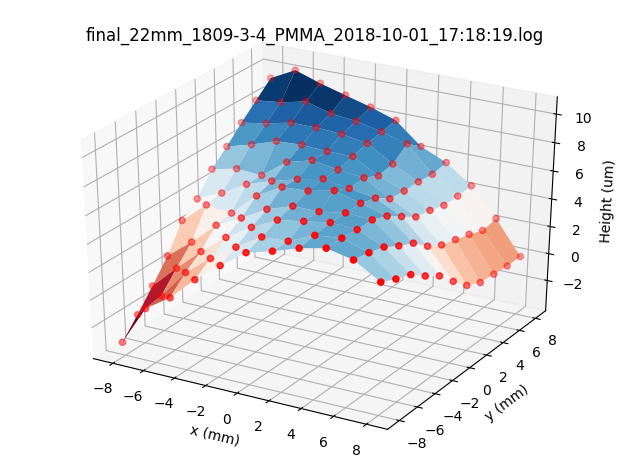
\includegraphics[width=0.5\linewidth]{appendix/figs/heightmap}
	\caption{}
	\label{fig:heightmap}
\end{figure}


\section{Stitching errors}

A few tips to reduce stitching errors in your pattern:
\begin{itemize}
	\item use height measurement
	\item minimize exposure time
		\begin{itemize}
		\item can you use negative instead of positive resist (or vice versa)?
		\item can you use a bigger beam?
		\end{itemize}
	\item smart placement of main fields in LayoutBeamer
		\begin{itemize}
		\item choose mainfield size in a suitable way
		\item choose "Floating" placement
		\item choose "Follow geometry" writing order
	\end{itemize}
	\item split off your stitching-sensitive parts from those you don't care so much about, and do separate exposures within one job
\end{itemize}


\references{dissertation}

